\begin{abstract}
	L'obiettivo dell'esperienza è la misura della costante  Boltzmann tramite la misura del rumore termico prodotto da resistenze di vari valori. Per effettuare questa misura sarà necessario amplificare notevolmente il rumore generato dalla resistenza e filtrarlo su una banda di frequenze in modo da poter ricavare $k_B$ a partire dalla formula di Nyquist del rumore termico.
\end{abstract}

\section{Strumentazione}
La strumentazione usata è quella presente sul banco di lavoro, più:
	\begin{itemize}
		\item un INA114 (precision instrumentation amplifier);
		\item due IC AD708 (ultra low offset dual op-amp);
		\item un AD736 (true rms-to-dc converter).
	\end{itemize}

Essendo il circuito realizzato molto sensibile ad eventuali rumori nell'effettuare i collegamenti su breadboard si è cercato di minimizzare gli effetti di induzione e 	si è montato il circuito in \figurename{ \ref{fig:prel}}.
Si è proceduto inoltre  a alimentare tutti i componenti con le medesime linee
	di distribuzione (tensioni $V_{+}= $ \SI{5.00(4)}{\volt} e $V_{-}= $ \SI{-5.01(4)}{\volt}).

	\begin{figure}[h]
		\begin{minipage}{0.65\textwidth}
			\centering
			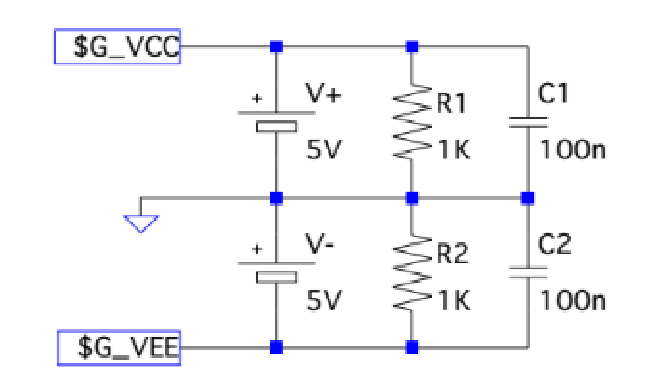
\includegraphics[scale=0.5]{prelim.png}
			\caption{Circuito di filtro per l'alimentazione.}
			\label{fig:prel}
		\end{minipage}
		\begin{minipage}{0.3\textwidth}
			\begin{tabular}{l@{ }c@{ }l}
				$R_{1}$& = &\SI{9.84(9)}{\kilo\ohm}\\
				$R_{2}$& = &\SI{9.74(9)}{\kilo\ohm}\\
				$C_1$& = &\SI{113(5)}{\nano\farad}\\
				$C_2$& = &\SI{106(5)}{\nano\farad}\\
			\end{tabular}
		\end{minipage}
	\end{figure}

\section{Metodo di misura}

	Per effettuare le misure è stato realizzato l'apparato in \figurename{ \ref{fig:completo}}
	verificando per ciascuno dei blocchi l'operatività.
	Effettuate tali verifiche sono stati collegati tra loro i vari blocchi
	e sono stati acquisiti i valori di tensione, $V_{RMS}$, letti in continua sul voltmetro,
	per vari valori di resistenze in dotazione.

	Dalla campionatura ottenuta attraverso un fit a tre parametri sono state ottenuti i valori
	di $V_{0n}$, $R_{T}$, $R_{n}$; rispettivamente : il rumore in uscita a resistenza nulla; la resistenza equivalente del rumore serie dell'amplificatore riferito all'ingresso ed il rapporto tra il rumore parallelo; il rumore serie dell’amplificatore, riferiti all’ingresso.

	\begin{figure}[h]
			\centering
			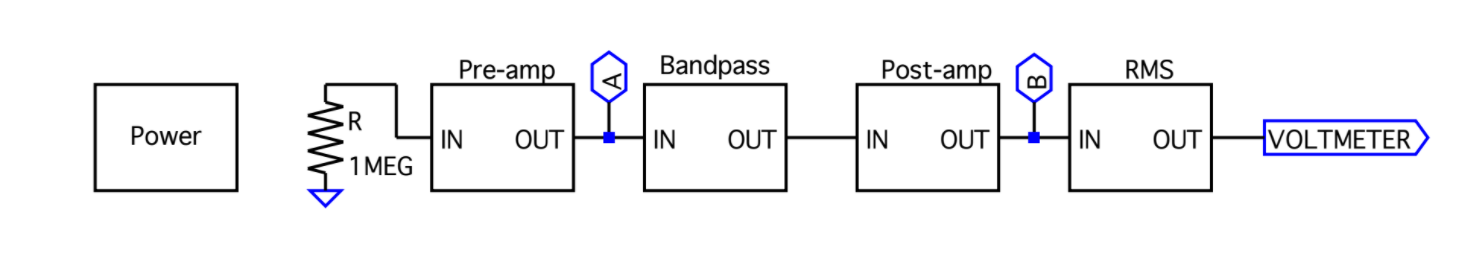
\includegraphics[scale = 0.4]{completo.png}
			\caption{schema dell'apparato di misura.}
			\label{fig:completo}
	\end{figure}

	Tali valori, essendo determinati da $k_{B}$ da relazioni descritte nel seguito, hanno permesso
	di ricavare una misura della costante di Boltzmann.
